\chapter{Implications of codon–anticodon interaction on the regulation of translation}

In the previous chapter I have shown that the codon usage and its interaction
with \trna anticodons remains remarkably stable across the variability of the
transcriptome during mammalian development.

Shortly after the publication of our research on \trna gene regulation during
mouse development, \citet{Gingold:2014} published \texttitle{A Dual Program for
Translation Regulation in Cellular Proliferation and Differentiation}. They
report that different programmes of cellular function preferentially use
different sets of codons, and that the pool of active \trna[s] adapts
dynamically to decode this set of codons with high efficiency.

Because its conclusions are highly relevant to our own research we evaluated the
paper carefully. In the following, I will first describe the paper’s main
findings, to the extent that they are relevant to our own research. I will then
outline our concerns with the analysis, and the subsequent experiments we
performed in an effort to explain how our previous results relate to this paper.

\section{“A dual program for translation regulation in cellular proliferation
and differentiation”}

\citet{Gingold:2014} investigated the abundance of \trna anticodons and the
codon usage of different groups of protein-coding genes in patient tissue
samples and human-derived cell lines in different cellular conditions --- five
primary cancers, induced differentiation, release from serum starvation,
senescence, and \gene{MYC} and \gene{RAS} overexpression --- with the aim of
characterising the differences in \trna gene expression and \trna anticodon
abundance. They hypothesise that the balance between \trna anticodon supply and
codon demand might influence the rate of production of proteins from \mrna
\citep{Gingold:2011}.

\subsection{\abbr{trna} anticodons change in abundance in tumour tissues}

Using microarray expression data for \trna genes, they show that there are
specific anticodon isoacceptors whose abundance changes reproducibly in specific
tumours (lymphomas), mirroring results reported previously
\citep{Pavon-Eternod:2009}.

\subsection{Codon usage differs between genes involved in cell proliferation and
genes involved in differentiation}

They then looked at protein coding genes within \go terms that they associated
with healthy, adult tissue (“pattern specification process”) and tumour tissue
(“M phase of mitotic cell cycle”). They show that the codon usage bias in these
two \go terms (averaged over all containing genes) clearly differs\todo{fig
2A?}.

They expand their analysis by calculating the mean codon usage across many \go
categories and perform \pca on the resulting matrix. This reveals that the
largest contributor to the variation stems from the split of the \go terms into
two distinct sets, one encompassing multi-cellular \go terms and the other cell
autonomous \go terms. They argue that these two sets of \go terms correspond to
\go terms functionally responsible for maintaining cell homoeostasis on the one
hand, and rapid cellular division, such as found in tumours, on the other hand.
In other words, different sets of codons are preferentially used in rapidly
dividing cells than in healthy cells.

\textfloat{go-cub-pca}{spill}
    {%
        \begin{minipage}{0.6\textwidth}
            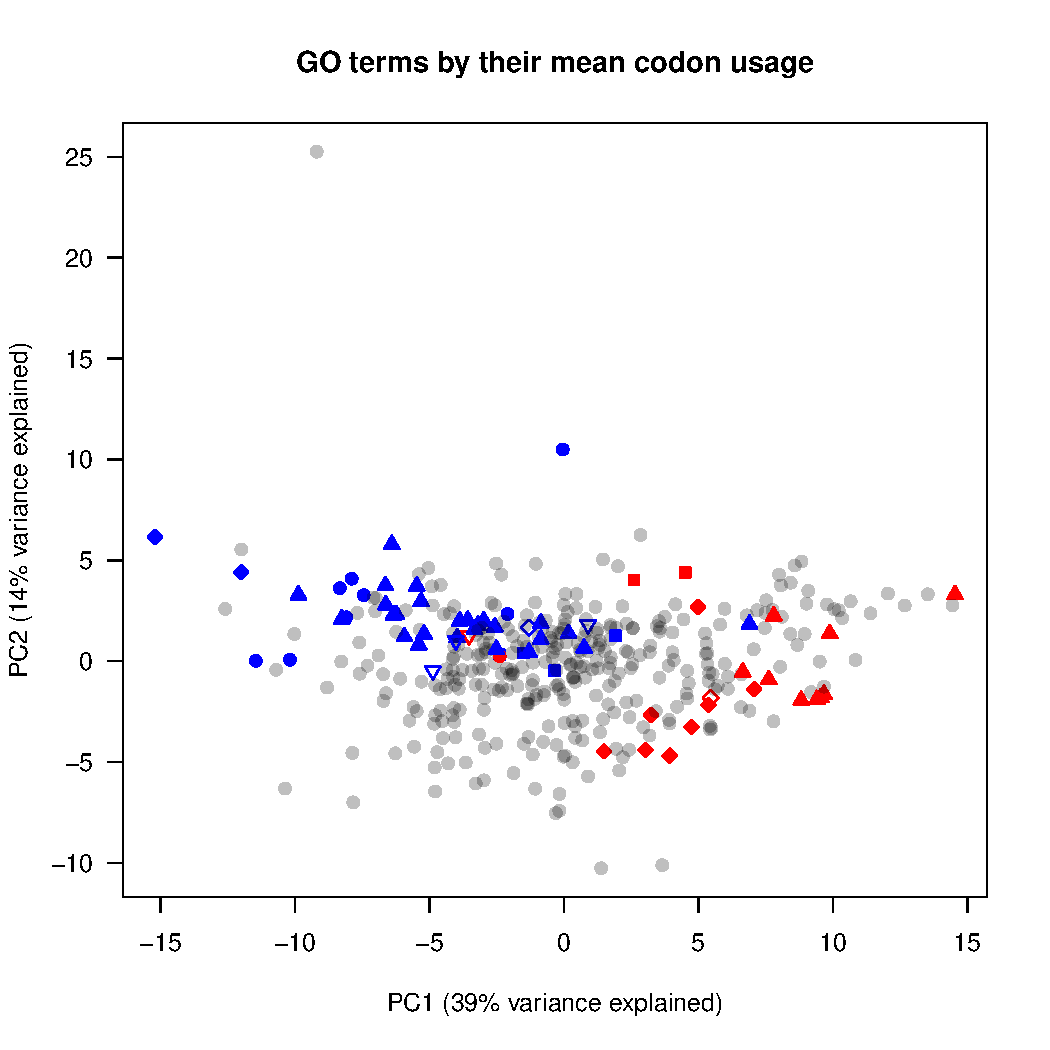
\includegraphics[width=\textwidth]{go-cub-pca}
        \end{minipage}%
        \begin{minipage}{0.4\textwidth}
            \begingroup
            \small\sffamily
            \begin{tabu} to \textwidth {@{}>{\color{blue}\(}c<{\)}X@{}}
                \toprule
                \multicolumn{2}{@{}l}{Multi-cellular} \\
                \midrule
                ▲ & Development \\
                ⬤ & Differentiation \\
                ⬛ & Cell adhesion \\
                ◆ & Pattern specification \\
                ◇ & Multicellular organism growth \\
                ▽ & Angiogenesis \\
                \midrule
            \end{tabu}
            \begin{tabu} to \textwidth {@{}>{\color{red}\(}c<{\)}X@{}}
                \multicolumn{2}{@{}l}{Cell autonomous} \\
                \midrule
                ▲ & Mitotic cell cycle \\
                ⬤ & Nucleosome assembly \\
                ⬛ & Chromatin remodelling/modification \\
                ◆ & Translation \\
                ◇ & \mrna metabolic process \\
                ▽ & Negative regulation of cell cycle \\
                \bottomrule
            \end{tabu}
            \endgroup
        \end{minipage}
    }
    {\pca of mean \go term codon usage.}
    {Each dot corresponds to one \go term. The position of the dots is derived
    by rotating the matrix of the mean codon usage of the genes belonging to
    each \go term. Created using methods of \citet{Gingold:2014} (the precise
    numbers differ slightly due to the use of different implementations to
    perform the analysis but this does not impact the interpretation).}

\subsection{Differential codon usage in cell-condition specific gene sets
matches \abbr{trna} anticodon abundance in corresponding cells}

Finally, \citet{Gingold:2014} use \rnaseq data of the previously mentioned cell
types to argue that gene expression changes do indeed correlate with the first
principal component of the \pca, with tumour samples showing more increased
expression towards the more we go towards the cell autonomous end of the axis,
and more decreased expression towards the multi-cellular end, and that this
trend is reversed for samples taken after induced differentiation using retinoic
acid. A similar analysis is then done for the expected translational efficiency,
by using \trna anticodon abundance to calculate the fold change of the \tai,
matched against the codon usage bias in the different \go terms. However, the
authors did not calculate correlations between the first principal component and
either the codon usage bias or the \tai fold change. Instead, they merely
visualised the presumed correspondence using a potentially misleading colour map
\citep{Borland:2007}. Furthermore, the absolute range of changes are minute
(range of \tai fold change \numrange{0.86}{0.905} in one case), and the lack of
statistical analysis makes it impossible to say whether these changes are in
fact significant, assuming they correlate at all (\cref{fig:gingold-fig-3c}).

\textfig{gingold-fig-3c}{body}{\textwidth}
    {Projection of the \trna and \mrna expression changes on the codon usage
    map.}
    {Both panels show the same \pca as in \cref{fig:go-cub-pca}. In the top
    panel, the colours correspond to the fold change in predicted translation
    efficiency of the genes constituting each \go term, given the change in
    cellular abundance of \trna anticodons compared to normal cells. The bottom
    panel shows the mean fold change in \mrna levels per \go term compared to
    normal cells. Figure from \citet{Gingold:2014}.}

\section{Are \abbr{trna} anticodon abundance and codon usage highly adapted to
different cellular conditions?}

To bring in line these two findings — the stability of the anticodon pool on the
one hand, and the malleability of the anticodon pool to match demand of highly
expressed on the other hand — we turned our attention to differences between
healthy tissue and tumour cell lines in \mmu and \hsa.

Since we were already in possession of relevant \trna data we decided to use our
own data to recapitulate these findings. A first observation was that while our
own research so far had looked at the whole transcriptome, \citet{Gingold:2014}
had looked at specific subsets. While both approaches are valid in their own
right, some caution is necessary when comparing the results: the smaller the set
of genes one looks at, the larger the effects of random sampling of the genes
become. When analysing a particular feature, such as the codon usage bias,
random sampling will thus contribute a larger part to the variation between two
small sets than between two large sets. If one wants to assert that deviations
are nonrandom, one thus has to account for this effect
(\cref{fig:sample-size-dependent-cub}).

\textfig{sample-size-dependent-cub}{spill}{\textwidth}
    {Dependence of codon usage variability on sample size.}
    {Genes were randomly sample from the human genome to create sets of sizes
    given by \(x\) (in grey). The mean codon usage of the sets was calculated,
    and their Pearson correlation to the genomic background is shown on the
    \(y\) axis. Overlaid are actual gene sets given by human \go categories.}

The plot illustrates that few \go categories, if any, can confidently be said to
have a codon usage varying more than just randomly. In addition, the allocation
of individual \go categories to either set can certainly also be criticised: It
is certainly not clear why “translation” should be more active during cellular
division than in stable cells. The authors rather describe the relevant set as
“cell autonomous” \go terms, but the paper’s argument implicitly assumes that
this corresponds to cell division. Furthermore, the allocation of genes to \go
terms was performed via simple textual matching, such that \go sub-categories
whose description contains the text “differentiation and proliferation” would be
counted as belonging to the \go super-category “differentiation”.

In order to test whether the anticodon pool does indeed adapt to specific
cellular conditions, we examined whether the matching codon--anticodon
adaptation (estimated via the translation efficiency index \tai) is higher
between matching \mrna and \trna transcriptomes than between mismatching ones.
In other words, we looked at the \mrna pool specific to cellular conditions, and
calculated the \tai[s] for
\begin{enumerate*}
    \item matching \trna pools, and
    \item mismatching \trna pools
\end{enumerate*}
(\cref{fig:tai-matching-mismatching}).

\textfig{tai-matching-mismatching}{spill}{0.8\textwidth}
    {\tai between matching and mismatching codon--anticodon pools.}
    {}

\todo[inline]{What is the result?}

Furthermore, the trend seen in \cref{fig:go-cub-pca} does in fact exist to the
same degree when plotting amino acid usage rather than codon usage
(\cref{fig:go-aa-pca}). This suggests that rather than being driven by \go term
function, both codon usage and amino acid usage changes are driven by some other
genomic feature. In fact, the first principal component in \cref{fig:go-cub-pca}
correlates almost perfectly with \gc bias (\cref{fig:cub-pc1-vs-gc}). The nature
of this relationship is still unclear, and needs to be explored in more detail.

\textfig{go-aa-pca}{body}{0.8\textwidth}
    {\pca of mean \go term amino acid usage.}
    {\todo{Add description}}

\textfig{cub-pc1-vs-gc}{body}{0.8\textwidth}
    {\gc bias against PC1 of the mean \go term codon usage bias \pca.}
    {\todo{Add description}}

Furthermore, if a mechanism leading to the adaptation of the cellular \trna pool
to different cellular conditions existed, we would expect this to be well
conserved across mammalian evolution. Indeed, such an effect should show a
\emph{stronger} conservation of the codon usage bias across different functional
gene categories than conservation of other genomic features, such as the \gc
bias. Using genome data from different mammalian species and homology
information for the annotated \go categories in humans, we can calculate the
respective conservation of codon usage on the one hand, and \gc bias on the
other hand. The result is summarised in \cref{fig:cub-conservation}.

\textfig{cub-conservation}{body}{0.8\textwidth}
    {Conservation of \go term specific codon bias}
    {}
